
%%%%%%%%%%%%%%%%%%%%%%% file typeinst.tex %%%%%%%%%%%%%%%%%%%%%%%%%
%
% This is the LaTeX source for the instructions to authors using
% the LaTeX document class 'llncs.cls' for contributions to
% the Lecture Notes in Computer Sciences series.
% http://www.springer.com/lncs       Springer Heidelberg 2006/05/04
%
% It may be used as a template for your own input - copy it
% to a new file with a new name and use it as the basis
% for your article.
%
% NB: the document class 'llncs' has its own and detailed documentation, see
% ftp://ftp.springer.de/data/pubftp/pub/tex/latex/llncs/latex2e/llncsdoc.pdf
%
%%%%%%%%%%%%%%%%%%%%%%%%%%%%%%%%%%%%%%%%%%%%%%%%%%%%%%%%%%%%%%%%%%%


\documentclass[runningheads,a4paper]{llncs}

\usepackage{amssymb}
\setcounter{tocdepth}{3}
\usepackage{graphicx}

\usepackage{url}
\urldef{\mailsa}\path|{alfred.hofmann, ursula.barth, ingrid.haas, frank.holzwarth,|
\urldef{\mailsb}\path|anna.kramer, leonie.kunz, christine.reiss, nicole.sator,|
\urldef{\mailsc}\path|erika.siebert-cole, peter.strasser, lncs}@springer.com|    
\newcommand{\keywords}[1]{\par\addvspace\baselineskip
\noindent\keywordname\enspace\ignorespaces#1}


\usepackage{listings}
\usepackage{xcolor}
\usepackage{textcomp}

\usepackage{selinput}
\SelectInputMappings{   % Semi-automatic determination
               % of input encoding
  oslash={ø},           % by a list of selected glyphs
	              % see: http://partners.adobe.com/public/developer/en/opentype/glyphlist.txt
}


\begin{document}

\mainmatter  % start of an individual contribution

% first the title is needed
\title{Project in Personal Data Interaction:\\FriendBump}

% a short form should be given in case it is too long for the running head
\titlerunning{Project in Personal Data Interaction: FriendBump}

% the name(s) of the author(s) follow(s) next
%
% NB: Chinese authors should write their first names(s) in front of
% their surnames. This ensures that the names appear correctly in
% the running heads and the author index.
%
\author{S\o ren Howe Gersager \and Anders L\o nberg Rahbek}
%
\authorrunning{Project in Personal Data Interaction: FriendBump}
% (feature abused for this document to repeat the title also on left hand pages)

% the affiliations are given next; don't give your e-mail address
% unless you accept that it will be published
\institute{DTU Compute, Technical University of Denmark, \\Richard Petersens Plads, Building 324, 2800 Kgs. Lyngby, Denmark \\
%\mailsa\\
%\mailsb\\
%\mailsc\\
\url{http://www.compute.dtu.dk/}}

%
% NB: a more complex sample for affiliations and the mapping to the
% corresponding authors can be found in the file "llncs.dem"
% (search for the string "\mainmatter" where a contribution starts).
% "llncs.dem" accompanies the document class "llncs.cls".
%

\toctitle{Lecture Notes in Computer Science}
\tocauthor{Authors' Instructions}
\maketitle


\begin{abstract}
The abstract should summarize the contents of the paper and should
contain at least 70 and at most 150 words. It should be written using the
\emph{abstract} environment.
\keywords{geolocation·android·prototyping·app}
\end{abstract}


\section*{Preface}
This report is produced based on a course project in Personal Data Interaction on the Technical University of Denmark. The references are stated with a number in brackets eg. [1]. If the reference is placed after the period in a section, the reference is used as reference for the entire section. 
Both authors are responsible for the entire content of this report.


\section{Introduction}
Many of us has tried to go shopping, been to a conference or a concert, where you came home and discovered that one of your friends had also been there. If you had known that he would be there, you could’ve met with him and possibly made the experience more enjoyable.\\

This leaves us with the following problem definition: You don’t know when a friend is nearby but you would like to know in certain situations. \\

This problem can be solved by a personal app, that allows you to  broadcasts your location to your friends and your friends location to you which enables you to quickly contact them when you are close to each other.\\

In this report we will describe the process of developing a prototype solution to solve this problem.
We start with related works to describe how our app differs from other similar solutions in the market. 
We analyse our problem further and then describe our design for the app. We evaluate the design, after describing the implementation. \\
Finally we go through our results and discuss them. Last, some remarks for possible future work on the app and a conclusion. 

\section{Analysis}
As the problem is, that you don’t know if a friend is nearby, the immediate solution would be to continuously broadcast your your location to your friends.
However we have to factor in privacy and avoid giving the users the feeling of being spied on, people will probably not use a solution that allows everyone to see their location at all times.\\
Also we figured the user should be able to disable broadcasts temporarily, because there are times when you don't want to advise your location, like going to the doctors or on a date where you’d rather be incognito. 

\section{Design}
Our design methods is divided into two overall parts: a low-fi prototype which is is developed based on an initial user story map and done with mock-ups, and a hi-fi prototype, an Android app. The hi-fi prototype is based on the low-fi prototype. \\

\subsection{Low-fi prototype}
We wanted to create a fixed-path prototype, which allowed for interaction by users early as explained in \cite{prototyping}. As a low-fi we used a mockup tool \cite{ninja}. The choice of this were to make it quick, but intuitive for our fellow students to understand, and thus give us better feedback. \\

We wanted to make the design as simple and direct as possible. The features we wanted, should be right at the fingertips, so you shouldn’t have to tap many times to get to the wanted function. 
We wanted the following: 
\begin{itemize}
  	\item A map to see where our friends are 
	\item A list with those friends to give the user a better overview over these friends. 
	\item A text-field which told the user how many friends that’s near him
	\item Markers in form of profile image from a social network
	\item An icon in the list, to show which network the friend is from
	\item Distance to each of the friends
	\item When (and maybe what) the friend has made an update on the particular social network.
	\item A button to toggle the broadcast on and off\\ 
\end{itemize}

All this is shown in figure 1. 

As functions we needed to could choose a friend, and then could call and sms this friend as well getting navigation to the friend - see figure 2. 

First were the list always visible (non-slide) but after a quick \& dirty evaluation (see evaluation), we changed it to a slide-list. This was to make the map bigger for the user, which is very important when it’s on a small screen - see figure 3. 

\subsection{Hi-fi prototype}

As the hi-fi prototype is based on the low-fi, we implemented the design from low-fi with the changes we mentioned last in latter subsection. 

We decided that our hi-fi prototype should be more vertical slice than the lo-fi, and thus focusing on making it show friends on a map, instead of including non-essential features. 

From some quick \& dirty and talk aloud evaluation, we made some changes and removed/added some things. 

\textbf{What we changed:}\begin{itemize}
\item Button to toggle broadcast on and off\\
We found out, that people didn’t understood the first icon (top-left icon on figure 1), so we found another icon based on suggestions from evaluation. \\


\textbf{What we removed:}
\item Updates from network\\
We removed this to make out prototype more vertical and because it was in general a little out of our scope. It was a nice feature but nothing more. \\

\item Text-field\\
We removed the text-field which told the user how many friend there was near him. The user can manage to count some few friend, and the other case with many friend, we found a possible solution using visualization (See section ). \\

\textbf{What we added:}
\item Call and SMS button \\
We added two buttons: a call button and a SMS button, so the user could call/SMS a friend directly from the app. 

\item PLACEHOLDER PATHFINDING

\end{itemize}

After further development and quick \& dirty, we changed the button to toggle the broadcast on and off and added a nudge button. We also removed updates from social networks. See figure 2 and hi-fi. 

The result can be viewed on figure 4. 

\section{Implementation}
Our implementation is divided into two parts: the already mentioned app and a backend server. The backend is composed of a python webserver and a RabbitMQ server\cite{rabbitmq}. \\
We will in the following section describe these two parts and details regarding them. 

\subsection{Android app}
Our activity has several functions, which are for communicating with the backend message-queue and common Android functionality. A table of these function and a short description, can be found in [ref] \\
There are a couple of non-trivial functions, which we will describe in a bit more detail below.\\

\underline{drawMarkerBitmap}\\
This function creates a bitmap object containing the initials of the person on a round and red background, for example Anders Rahbek turns into AR.\\

This is used to show an unique marker for a friend, thus the function is been called from “updateMarker” function. \\
The function drawing the bitmap to the marker is taken from Stack Overflow\cite{bitmapstackoverflow}

\underline{getNumber}\\
The getNumber function, tries to find a telephone number based on a name. It iterate through the mobiles phonebook and return the number if it finds the name, null otherwise. \\

The function is used to create an action to a notification, so the user can call the friend directly from the notification. It is also used to call and sms from the list, under a person. 
The code is strong inspired of the code from \cite{number}.\\


To give a sense on how some of the functions work together, we have made some sequence diagrams, to show the flow. These diagrams is [ref]\\ 

For the app we used the following libraries: Paho MQTT\cite{paho}, Sothee Sliding up panel\cite{slidinguppanel}.


\subsection{Backend (RabbitMQ and Flask)}
The Python web server is running a simple Flask[ref] script which can be queried with an email and then returns a list of predetermined friends in JSON format, we decided to use these tools because they allowed us to quickly set up a “mock” backend for the app to communicate with. While testing the app among a number of users, we simply modified the script to return a number of their chosen friends based on their email.\\

The RabbitMQ is responsible for acting as a message queue for relaying the messages between devices running the app. The protocol used for the messages is MQTT, which was chosen because it’s lightweight in terms of code footprint and network bandwidth. The message queue use the notion of “topics”, so each message is broadcast on a topic, which in our case is the email of the user and the latitude and longitude of their location reduced to 2 decimal places. This reduces the number of updates received by the app since you do not receive an update from a friend if your location is not the same as theirs to 2 decimal places. In hindsight this could also be implemented server-side where the server compared the last location with all friends, and only relayed it if they were within radius of each other.

 
\section{Related works}
\textbf{Find My Friends \& Buddies by Sygic - FMFB (updated 2014, Google Play, free)}\\
This is an app for locating your friends in real-time much like our app. What is different is the built-in minimum radius our app has, thus you are not able to see your friends location at all times. Furthermore FMFB allows you to see the movement of your friends for the last week, this is intrusive in our opinion and we do not allow that.\\

\textbf{Family Locator by Life360 (updated 2015, Google Play, Free)}\\
Family Locator is similar to our app in the sense that it allows you to see the location of other people, the way ours differ is that their solution are marketed to families or more precisely parents who want to get updated on their children's location, and thus they are also able to see their positions at all times. 


\section{Evaluation}
\subsection*{Quick \& dirty}

\subsection*{Think aloud}
We conducted the Think aloud feedback session because we wanted to assess the usability of our design. The session was conducted on our hi-fi prototype in an outdoors context to simulate a natural situation our app might be used in.\\

We  have defined the following tasks for our prototypes:\\
\begin{itemize}
\item Can the user track and find a friend? 
\item Can the user turn on/off location broadcasts? 
\item Can the user track a friend from a notification?
\item Can the user message/call/nudge a friend from a notification?
\item Can the user asses the distance from a given user?
\end{itemize}

\section{Result}
\section{Discussion}
We would like to have used at least five evaluators for the heuristic evaluation as a larger number of evaluators finds more usability problems as J. Nielsen and R. Molic (1990) found.\cite{heuristics}
Due to our "improvised" backend, for calling and texting a friend, the app makes the assumption that the friend is located in the phone book with the same name it receives from the backend. 
\section{Future work}
\section{Conclusions}

\begin{thebibliography}{4}

\bibitem{prototyping} M. Beaudouin-Lafon, W. Mackay: Prototyping Tools and Techniques
\bibitem{paho} Paho Project: URL \url{http://eclipse.org/paho/}
\bibitem{slidinguppanel} Android Sliding Up Panel: Github \url{https://github.com/umano/AndroidSlidingUpPanel}
\bibitem{nielsenheuristics}Refined heuristics of J. Nielsen: URL \url{http://www.nngroup.com/articles/ten-usability-heuristics/}
\bibitem{bitmapstackoverflow} Drawing a bitmap on a marker: URL \url{http://stackoverflow.com/questions/18335642/how-to-draw-text-in-default-marker-of-google-map-v2}
\bibitem{ninja} NinjaMock - Mockup tool: URL \url{http://ninjamock.com}
\bibitem{rabbitmq} RabbitMQ - Message Queue Server: URL \url{http://www.rabbitmq.com/}
\bibitem{heuristics}Nielsen, J., and R. Molich. “Heuristic Evaluation of User Interfaces.” SIGCHI Bulletin (1990): 249–256. Print.
\bibitem{number} Search for number in phonebook by name: URL \url{http://stackoverflow.com/questions/18201108/getting-number-and-names-of-contacts-in-android}
% bibliography examples:

%\bibitem{proceeding2} Foster, I., Kesselman, C., Nick, J., Tuecke, S.: The Physiology of the
%Grid: an Open Grid Services Architecture for Distributed Systems
%Integration. Technical report, Global Grid Forum (2002)

%\bibitem{url} National Center for Biotechnology Information, \url{http://www.ncbi.nlm.nih.gov}

\end{thebibliography}


\section*{Appendix}

\subsection*{Transcript of summative think aloud evaluation}
The following \textit{in italic} is the transcript of the recordings of what the evaluator has "thought". The question/task that the observer has given the evaluator, is the following bulletpoints. 

It's worth mentioned that the evaluator were used to use  an iPhone and not Android. \\

The evaluator is from now on denoted 'E'. \\
\begin{enumerate}
	\item \textbf{Track friend from notificaton}\\
		{[} The notification arriving{]} \\
		\textit{There is a notification...}\\
		{[}E pressing the notification and asking what the task was, for confirming it.{]}\\
		\textit{I can see S\o ren right next to me}\\
		
	\item \textbf{Call a friend directly from a notification}\\
		{[}The notification arriving{]} \\
		\textit{There is a notification. S\o ren is near me. The come some information up, if I long-pressing on the notification}\\
		
		{[}E is stopping and don't know what to do.{]}\\
	
	\item \textbf{SMS a friend from the app}\\
		{[}E has the app open from start{]}\\
		\textit{I pull up the list. Find S\o ren, pressing the little SMS-icon}\\
		{[}The default SMS app turns up{]}\\
		\textit{And I'm writing a SMS}\\
		
	\item \textbf{Nudge a friend from the app}\\
		{[}E has the app open from start{]}\\
		\textit{I pull up the friend-list. Ehm... Pressing on S\o ren. Then the little finger-icon}\\
		
	\item \textbf{Call a friend from the app}\\
		{[}E has the app open from start{]}\\
		\textit{I have the app in my hand. I pull up the friend-list. Pressing on S\o ren and pressing on the phone-icon}\\
		
	\item \textbf{Read the distance to a friend, from the app}\\
		{[}E has the app open from start{]}\\
		\textit{I can see S\o ren on the map. I pull up the friend-list. And then I can see the he is approx. 22 meters away.}\\
		
	\item \textbf{Turn broadcast off}\\
		{[}E has the app open from start{]}\\
		\textit{I orient myself around in the app. I pull up the friend-list. Pull it down again. I'm pressing the icon in the upper-right corner. Pressing on the sound-icon... a few times. \\I don't know.}
		
\end{enumerate}

\subsection*{Heuristic evaluation}
In the last iteration we have evaluated the app using the Nielsen heuristics[ref].

We have tested the interface independently using two evaluators, below is a summary of the issues found.\\



\begin{enumerate}
  \item \textbf{Visibility of system status}\\
  Our app keeps the user informed about the status of the app, through visual cues and Android Toast messages, however currently two things can be improved in the app regarding system status:
  \begin{enumerate}
    \item \textbf{Broadcast toggling}\\
    Right now the broadcast icon simply changes when toggling broadcasting, this could be improved further by using a Toast and maybe a more visual approach than the icon changes we use now, like adding a small animation to the icon change when touched, providing a sort of tactile feedback to the user.
    
    \item \textbf{Connectivity problems}\\
    The user can be notified of connectivity problems using Toasts and visual cues. 
We previously used a toast when failing to connect, but it was simply annoying rather than informative if a Toast pop-up every few seconds, telling the user it can’t connect. A timeout could be added, so it can only pop-up once every 5 minutes for example, even better a visual effect could be added so the user is constantly aware of the connectivity of the app, perhaps change the opacity of the screen or make it black and white with a visual indicator that it’s reconnecting.  
  \end{enumerate}
  \item \textbf{Match between system and the real world
}\\
Our app provides the user with system information in a clear, non-domain specific language. For example if the user tries to call the friend from the app and it can’t find the number it simple says \\
"Number not found. Can't make the call!".\\
This also happens with SMS and nudge.
  \item \textbf{User control and freedom}\\
  The sliding up bar can perhaps be activated by mistake, an icon with arrows facing up when slid down and down when slid up, could perhaps make the affordance more clear.
  \item \textbf{Consistency and standards}\\
  For the most, we using platform standards for our function. Some examples is the call and SMS functions. Here we used standard icons for these functions. 
As mentioned earlier in the Think-aloud evaluation, we need to change the icon for the broadcast button. The suggested solution is also more platform standardized than the current icon. \\
This could also been the case with the nudge function. The current icon is chosen so it’s not the same as the facebook nudge in order to avoid that the user thinks it’s the real facebook nudge function. But maybe there could be developed a even better and more clear icon than the current.
\item \textbf{Error prevention}\\
The calling or texting features in our app makes the assumption that the contact can be found with that precise name in the phone book, this is obviously an error-prone condition, this would not be an issue with a proper backend for handling user information.
\item \textbf{Recognition rather than recall}\\
The only thing our user has to recall, is where he can slide up the friend list and where he can make a call/SMS/nudge to a friend. There isn’t any straightforward solution to make it recognizable, without an error prevention problem occurs.
\item \textbf{Flexibility and efficiency of use}\\
In our apps current state we have no accelerators of any kind, however it would be ideal to add an accelerator for the marker of a friend so it automatically opens up the friend list with the given friends menu expanded, this would reduce the number of taps needed to access the friend functions and reduce the cognitive load of locating the friend in the list.
\item \textbf{Aesthetic and minimalist design
}\\
Our design is very minimalistic, so it’s quite easy to use. The reason for this is of cause partly to the vertical approach. 
Aesthetic wise we have some way to go. We need to make it more flat design so it complies with Android's material design patterns.
We decided to make the options for each friend in the friend list collapsable, as to not make it compete with other information on the screen.
\item \textbf{Help user to recognize, diagnose and recover from error}\\
While our feedback messages indicate the problems in plain language, they lack suggesting a solution, for example "Number not found. Can't make the call" could express that the contacts number needs to be added.
\item \textbf{Help and documentation}\\
We haven’t any help or documentation for the user at this moment. It would be ideal to make a guided tour of the app first time using it, to introduce the basic features of the app. 


\end{enumerate}


\begin{figure}
\centering
\caption{lo-fi prototype iteration 1}
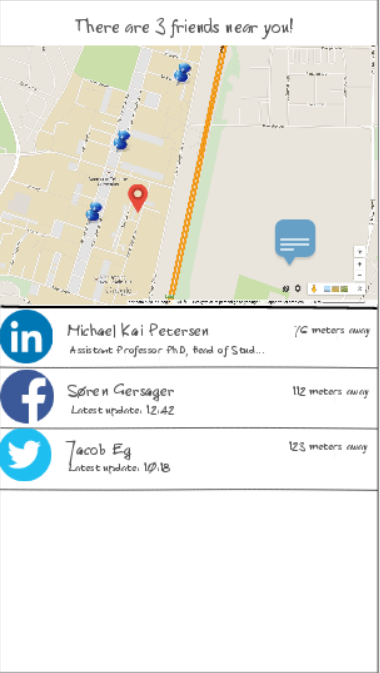
\includegraphics[width=0.6\textwidth]{figures/lo-fi-4}
\end{figure}

\begin{figure}
\centering
\caption{lo-fi prototype iteration 2}
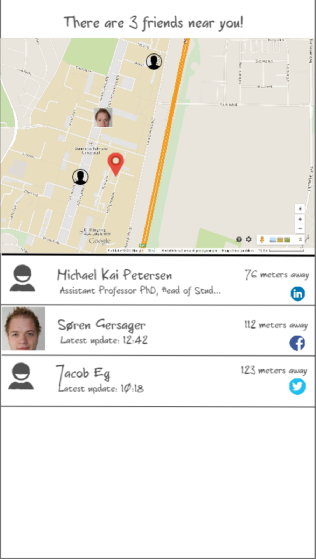
\includegraphics[width=0.6\textwidth]{figures/lo-fi-3}
\end{figure}

\begin{figure}
\centering
\caption{lo-fi prototype iteration 3, panel collapsed}
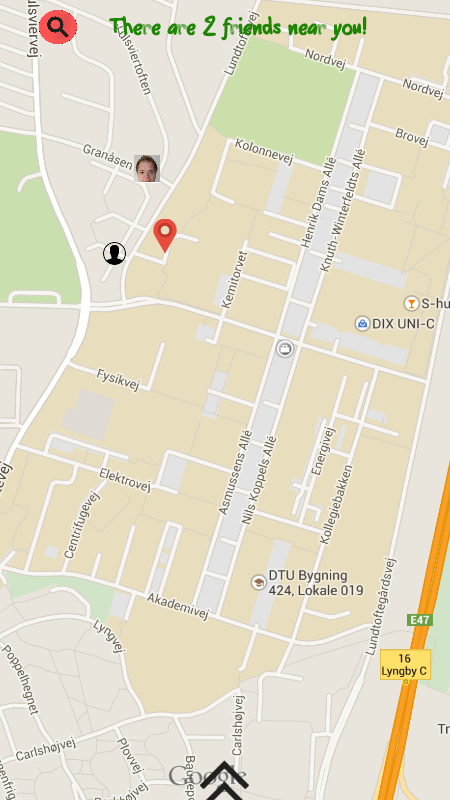
\includegraphics[width=0.6\textwidth]{figures/lo-fi-2}
\end{figure}

\begin{figure}
\centering
\caption{lo-fi prototype iteration 3, panel expanded}
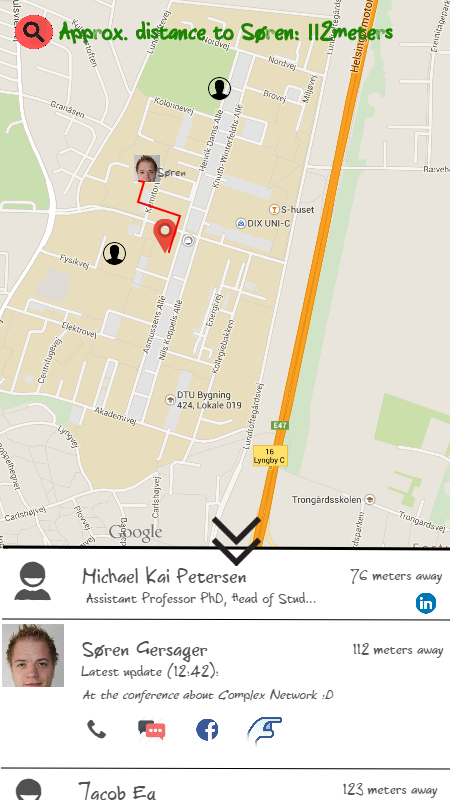
\includegraphics[width=0.6\textwidth]{figures/lo-fi-1}
\end{figure}

\subsection*{Sourcecode}
\lstset{numbers=left,
tabsize=2, numbersep=10pt,
  title=\lstname }
\lstinputlisting[language=Java]{FriendBump/mobile/src/main/java/com/example/syre/friendbump/MainActivity.java}
\end{document}
